%%%TNabcd
\begin{ex}%%Cau 1
	\immini[thm]{
		Cho hàm số $y=f(x)$ có đồ thị như hình bên. Hàm số $y=f(x)$ đồng biến trên khoảng nào?
		\choice
		{$(-1;1)$}
		{$(-\infty;-1)$}
		{$(2;+\infty)$}
		{\True $(0;2)$}
	}{
		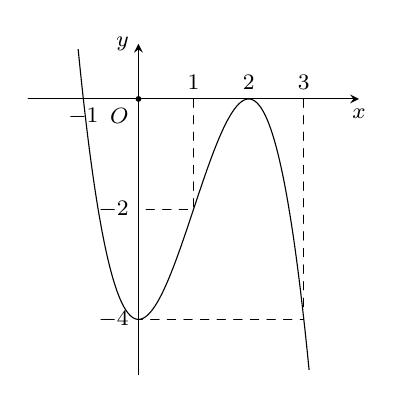
\begin{tikzpicture}[line join=round,line cap=round,>=stealth,font=\footnotesize,scale=0.7,declare function={f(\x)=-(\x)^3+3*(\x)^2-4;}]
			\def\xt{-2} \def\xp{4} \def\yd{-5} \def\yt{1}
			\draw[->] (\xt,0)--(\xp,0) node[below]{$x$};
			\draw[->] (0,\yd)--(0,\yt) node[left]{$y$};
			\fill (0,0) circle (1.5pt) node[below left]{$O$};
			\draw[dashed] (1,0)--(1,-2)--(0,-2) (3,0)--(3,-4)--(0,-4);
			\begin{scope}
				\clip (\xt+0.1,\yd+0.1) rectangle (\xp-0.1,\yt-0.1);
				\draw[samples=150,smooth,domain=\xt:\xp] plot(\x,{f(\x)});
			\end{scope}
			\node[below] at (-1,0) {$-1$};
			\foreach \x in {1,2,3} \node[above] at (\x,0) {$\x$};
			\foreach \y in {-2,-4} \node[left] at (0,\y) {$\y$};
		\end{tikzpicture}
	}
	\loigiai{
		Dựa vào đồ thị, ta thấy trên khoảng $(0;2)$ đồ thị hàm số đi lên từ trái sang phải. \\
		Do đó, hàm số đồng biến trên khoảng $(0;2)$.
	}
\end{ex}

\begin{ex}%%Cau 2
	\immini[thm]{
		Cho hàm số $y=f(x)$ có bảng biến thiên như hình. Giá trị cực tiểu của hàm số bằng
		\choice
		{$2$}
		{$-2$}
		{\True $4$}
		{$-4$}
	}{
		
\begin{tikzpicture}[>=stealth]
			\tkzTabInit[nocadre=false,lgt=1,espcl=2,deltacl=0.5]{$x$/.7,$y'$/.7,$y$/2.5}
			{$-\infty$, $-2$, $0$, $2$, $+\infty$}
			\tkzTabLine{ , +, $0$, -, d, -, $0$, +, }
			\tkzTabVar{-/$-\infty$, +/$-4$, -D+/$-\infty$/$+\infty$, -/$4$, +/$+\infty$}
		\end{tikzpicture}
	}
	\loigiai{
		Dựa vào bảng biến thiên, hàm số đạt cực tiểu tại $x = 2$ và giá trị cực tiểu của hàm số là $y_{\text{CT}} = 4$.
	}
\end{ex}

\begin{ex}%%Cau 3
	\immini[thm]{
		Đường cong ở hình vẽ bên là của đồ thị hàm số nào dưới đây?
		\choice
		{\True $y=-x^3+3x+1$}
		{$y=x^3-3x+1$}
		{$y=x^3-3x^2+1$}
		{$y=-x^3+3x-1$}
	}{
			\begin{tikzpicture}[line join=round, line cap=round, >=stealth, font=\footnotesize, declare function={f(\x)=-\x^3+3*\x+1;}]
			\def\xt{-2.8} \def\xp{2.2} \def\yd{-1.5} \def\yt{4}
			\draw[->] (\xt,0)--(\xp,0) node[above]{$x$};
			\draw[->] (0,\yd)--(0,\yt) node[right]{$y$};
			\fill (0,0) circle (1.5pt) node[below right]{$O$};
			
			\draw (-1,0) node[above]{$-1$};
			\draw (1,0) node[below]{$1$};
			\draw (0,3) node[left]{$3$};
			\draw (0,-1) node[right]{$-1$};
			
			\draw[dashed] (-1,0)--(-1,-1)--(0,-1);
			\draw[dashed] (1,0)--(1,3)--(0,3);
			
			\begin{scope}
				\clip (\xt+0.1,\yd+0.1) rectangle (\xp-0.1,\yt-0.1);
				\draw[samples=150,smooth,domain=\xt:\xp] plot(\x,{f(\x)});
			\end{scope}
		\end{tikzpicture}
	}
	\loigiai{
		Dựa vào hình dáng, ta thấy đây là đồ thị của hàm số bậc ba $y=ax^3+bx^2+cx+d$ với hệ số $a<0$. Từ đó loại phương án $y=x^3-3x+1$ và $y=x^3-3x^2+1$.\\
		Đồ thị hàm số đi qua điểm $(0;1)$ nên tung độ gốc bằng $1$. Do đó loại phương án $y=-x^3+3x-1$.\\
		Vậy hàm số cần tìm là $y=-x^3+3x+1$.
	}
\end{ex}

\begin{ex}%%Cau 4
	Cho hàm số $y=-x+1-\dfrac{3}{2x-4}$. Phương trình đường tiệm cận xiên của đồ thị hàm số đã cho là
	\choice
	{$y=x-1$}
	{\True $y=-x+1$}
	{$y=-x-1$}
	{$x=2$}
	\loigiai{
		Ta có $\lim\limits_{x\to +\infty} \left[ y - (-x+1) \right] = \lim\limits_{x\to +\infty} \left( -\dfrac{3}{2x-4} \right) = 0$ và $\lim\limits_{x\to -\infty} \left[ y - (-x+1) \right] = \lim\limits_{x\to -\infty} \left( -\dfrac{3}{2x-4} \right) = 0$.\\
		Do đó, đường thẳng $y=-x+1$ là tiệm cận xiên của đồ thị hàm số đã cho.
	}
\end{ex}

\begin{ex}%%Cau 5
	Cho hàm số $y=\dfrac{x^2-3x+1}{x-1}$ có đồ thị là $(C)$. Điểm nào dưới đây thuộc đồ thị $(C)$?
	\choice
	{\True $M(2;-1)$}
	{$N(0;1)$}
	{$Q(-1;3)$}
	{$P(3;2)$}
	\loigiai{
		Thay tọa độ điểm $M(2;-1)$ vào hàm số, ta có $-1 = \dfrac{2^2-3\cdot 2+1}{2-1} = \dfrac{-1}{1} = -1$ (thỏa mãn).\\
		Vậy điểm $M(2;-1)$ thuộc đồ thị $(C)$.
	}
\end{ex}

\begin{ex}%%Cau 6
	\immini[thm]{
		Cho hàm số $y = f(x)$ có bảng biến thiên như hình bên. Số nghiệm thực của phương trình $2f(x)+3=0$ là
		\choice
		{$2$}
		{$0$}
		{$1$}
		{\True $3$}
	}{
		
\begin{tikzpicture}[>=stealth]
			\tkzTabInit[nocadre=false,lgt=1.2,espcl=2,deltacl=0.5]{$x$/.7,$f'(x)$/.7,$f(x)$/2}
			{$-\infty$, $-1$, $2$, $+\infty$}
			\tkzTabLine{ , +, $0$, -, $0$, +, }
			\tkzTabVar{-/$-\infty$, +/$2$, -/$-2$, +/$+\infty$}
		\end{tikzpicture}
	}
	\loigiai{
		Ta có $2f(x)+3=0 \Leftrightarrow f(x) = -\dfrac{3}{2}$.\\
		Số nghiệm của phương trình đã cho là số giao điểm của đồ thị hàm số $y = f(x)$ và đường thẳng nằm ngang $y = -\dfrac{3}{2}$.\\
		Dựa vào bảng biến thiên, ta thấy đường thẳng $y = -\dfrac{3}{2}$ cắt đồ thị hàm số $y = f(x)$ tại $3$ điểm phân biệt (do $-2 < -\dfrac{3}{2} < 2$).\\
		Vậy phương trình đã cho có $3$ nghiệm thực.
	}
\end{ex}

\begin{ex}%%Cau 7
	\immini[thm]{
		Hình vẽ sau là đồ thị của hàm số
		\choice
		{$y=\dfrac{-x-3}{x+1}$}
		{$y=\dfrac{x-3}{x-1}$}
		{\True $y=\dfrac{x+3}{x+1}$}
		{$y=\dfrac{x+3}{x-1}$}
	}{
		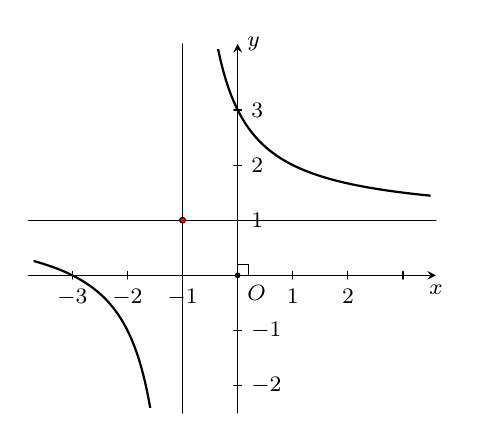
\begin{tikzpicture}[line join=round,line cap=round,>=stealth,font=\footnotesize,scale=0.7,declare function={f(\x)=(\x+3)/(\x+1);}]
			\def\xt{-3.8} \def\xp{3.6} \def\yd{-2.5} \def\yt{4.2}
			\draw[->] (\xt,0)--(\xp,0) node[below]{$x$};
			\draw[->] (0,\yd)--(0,\yt) node[right]{$y$};
			\fill (0,0) circle (1.5pt) node[below right]{$O$};
			\draw (0.2,0)|-(0,0.2);
			\draw (\xt,1)--(\xp,1) (-1,\yd)--(-1,\yt);
			\filldraw[fill=red,draw=black] (-1,1) circle (1.5pt);
			\foreach \x in {-3,-2,-1,1,2,3} \draw (\x,2pt)--(\x,-2pt);
			\foreach \x in {-3,-2,-1,1,2} \node[below] at (\x,-2pt) {$\x$};
			\foreach \y in {-2,-1,1,2,3} \draw (2pt,\y)--(-2pt,\y);
			\foreach \y in {-2,-1,1,2,3} \node[right] at (2pt,\y) {$\y$};
			\begin{scope}
				\clip (\xt+0.1,\yd+0.1) rectangle (\xp-0.1,\yt-0.1);
				\draw[thick,samples=150,smooth,domain=\xt:-1.15] plot(\x,{f(\x)});
				\draw[thick,samples=150,smooth,domain=-0.85:\xp] plot(\x,{f(\x)});
			\end{scope}
		\end{tikzpicture}
	}
	\loigiai{
		Dựa vào đồ thị hàm số ta thấy:
		\begin{itemize}
			\item Đồ thị có tiệm cận đứng là đường thẳng $x=-1$. Suy ra loại phương án $y=\dfrac{x-3}{x-1}$ và $y=\dfrac{x+3}{x-1}$.
			\item Đồ thị có tiệm cận ngang là đường thẳng $y=-1$. Suy ra loại phương án $y=\dfrac{x+3}{x+1}$.
			\item Đồ thị đi qua điểm $(0;-3)$ và $(-3;0)$. Hàm số $y=\dfrac{-x-3}{x+1}$ thỏa mãn.
		\end{itemize}
		Vậy đồ thị đã cho là của hàm số $y=\dfrac{-x-3}{x+1}$.
	}
\end{ex}

\begin{ex}%%Cau 8
	Cho hàm số $y=f(x)$ liên tục trên $\mathbb{R}$ và có bảng xét dấu đạo hàm như hình vẽ
	\begin{center}
		
\begin{tikzpicture}[>=stealth]
			\tkzTabInit[nocadre=false,lgt=1.2,espcl=2,deltacl=0.5]{$x$/.7,$f'(x)$/.7}
			{$-\infty$, $-1$, $0$, $2$, $4$, $+\infty$}
			\tkzTabLine{ , +, $0$, -, d, +, $0$, -, $0$, +, }
		\end{tikzpicture}
	\end{center}
	Đồ thị hàm số $y=f(x)$ có tất cả bao nhiêu điểm cực trị?
	\choice
	{$2$}
	{$1$}
	{\True $4$}
	{$3$}
	\loigiai{
		Hàm số $y=f(x)$ liên tục trên $\mathbb{R}$ và có đạo hàm $f'(x)$ đổi dấu $4$ lần khi qua các điểm $x=-1$, $x=0$, $x=2$, $x=4$. do đó đồ thị hàm số $y=f(x)$ có tất cả $4$ điểm cực trị.
	}
\end{ex}

\begin{ex}%%Cau 9
	Tiệm cận ngang của đồ thị hàm số $y=\dfrac{5x-1}{x+1}$ là đường thẳng có phương trình
	\choice
	{\True $y=5$}
	{$y=1$}
	{$y=-1$}
	{$y=-5$}
	\loigiai{
		Ta có $\lim\limits_{x\to +\infty} y = \lim\limits_{x\to +\infty} \dfrac{5x-1}{x+1} = 5$ và $\lim\limits_{x\to -\infty} y = \lim\limits_{x\to -\infty} \dfrac{5x-1}{x+1} = 5$.\\
		Vậy đồ thị hàm số có tiệm cận ngang là đường thẳng $y=5$.
	}
\end{ex}

\begin{ex}%%Cau 10
	Giá trị lớn nhất của hàm số $y=\dfrac{3x-1}{x-3}$ trên đoạn $[0;2]$ là
	\choice
	{\True $\dfrac{1}{3}$}
	{$5$}
	{$-5$}
	{$\dfrac{-1}{3}$}
	\loigiai{
		Hàm số $y=\dfrac{3x-1}{x-3}$ xác định và liên tục trên đoạn $[0;2]$.\\
		Ta có $y'=\dfrac{-8}{(x-3)^2} < 0$, $\forall x\in [0;2]$.\\
		Suy ra hàm số nghịch biến trên đoạn $[0;2]$.\\
		Vậy $\max\limits_{[0;2]} y = y(0) = \dfrac{1}{3}$.
	}
\end{ex}

\begin{ex}%%Cau 11
	Hàm số $y=-x^3+12x+5$ nghịch biến trên khoảng nào sau đây?
	\choice
	{$(-2;2)$}
	{$(-\infty;-1)$}
	{$(-3;0)$}
	{\True $(2;+\infty)$}
	\loigiai{
		Tập xác định: $\mathscr{D} = \mathbb{R}$.\\
		Ta có $y' = -3x^2+12$.\\
		$y' < 0 \Leftrightarrow -3x^2+12 < 0 \Leftrightarrow \hoac{&x<-2\\&x>2.}$\\
		Vậy hàm số nghịch biến trên các khoảng $(-\infty;-2)$ và $(2;+\infty)$.\\
		Đối chiếu với các phương án, hàm số nghịch biến trên khoảng $(2;+\infty)$.
	}
\end{ex}

\begin{ex}%%Cau 12
	\immini[thm]{
		Cho hàm số $f(x)$ liên tục trên $[-1;3]$ và có đồ thị như hình vẽ bên. Gọi $M$, $m$ lần lượt là giá trị lớn nhất và giá trị nhỏ nhất của hàm số $y=f(x)$ trên $[-1;3]$. Ta có giá trị của $M+2m$ là
		\choice
		{$M+2m=4$}
		{$M+2m=3$}
		{\True $M+2m=2$}
		{$M+2m=1$}
	}{
		\begin{tikzpicture}[line join=round, line cap=round, >=stealth, font=\footnotesize, declare function={f(\x)=(\x<0)*(2*\x+1) + (\x>=0)*((\x-1)^2);}]
			\def\xt{-1.8} \def\xp{4.2} \def\yd{-1.5} \def\yt{4.5}
			\draw[->] (\xt,0)--(\xp,0) node[below]{$x$};
			\draw[->] (0,\yd)--(0,\yt) node[left]{$y$};
			\fill (0,0) circle (1.5pt) node[below right]{$O$};
			
			\draw (-1,0) node[above left]{$-1$};
			\draw (1,0) node[below]{$1$};
			\draw (3,0) node[below]{$3$};
			
			\draw (0,4) node[left]{$4$};
			\draw (0,1) node[right]{$1$};
			\draw (0,-1) node[right]{$-1$};
			
			\draw[dashed] (3,0)--(3,4)--(0,4);
			\draw[dashed] (-1,0)--(-1,-1)--(0,-1);
			
			\begin{scope}
				\clip (\xt+0.1,\yd+0.1) rectangle (\xp-0.1,\yt-0.1);
				\draw[samples=150,smooth,domain=-1:3] plot(\x,{f(\x)});
			\end{scope}
			
			\draw (3.5,4) node[right]{$y=f(x)$};
		\end{tikzpicture}
	}
	\loigiai{
		Dựa vào đồ thị hàm số trên đoạn $[-1;3]$, ta có:
		\begin{itemize}
			\item Giá trị lớn nhất của hàm số là $M = \max\limits_{[-1;3]} f(x) = f(3) = 4$.
			\item Giá trị nhỏ nhất của hàm số là $m = \min\limits_{[-1;3]} f(x) = f(-1) = -1$.
		\end{itemize}
		Do đó, $M+2m = 4+2\cdot (-1) = 2$.
	}
\end{ex}

%%%Dung-Sai
\setcounter{ex}{0}
\begin{ex}%%Cau 1
	Cho hàm số $y=\dfrac{2x+1}{x-3}$ có đồ thị là $(C)$.
	\choiceTF
	{\True Đồ thị $(C)$ có tâm đối xứng là $I(3;2)$}
	{Hàm số đã cho nghịch biến trên $\mathbb{R}\setminus \{3\}$}
	{\True Đồ thị $(C)$ có đường tiệm cận đứng là $x=3$}
	{\True Giá trị lớn nhất của hàm số trên $[1;2]$ là $f(1)$}
	\loigiai{
		Tập xác định của hàm số là $\mathscr{D} = \mathbb{R} \setminus \{3\}$.\\
		Ta có $y' = \dfrac{2 \cdot (-3) - 1 \cdot 1}{(x-3)^2} = \dfrac{-7}{(x-3)^2} < 0, \forall x \in \mathscr{D}$.\\
		Suy ra hàm số nghịch biến trên các khoảng $(-\infty; 3)$ và $(3; +\infty)$.
		\begin{itemchoice}
			\itemch Đồ thị hàm số có đường tiệm cận đứng là $x=3$ và đường tiệm cận ngang là $y=2$.\\
			Do đó, tâm đối xứng của đồ thị $(C)$ là giao điểm của hai đường tiệm cận $I(3;2)$. Mệnh đề đúng.
			\itemch Hàm số nghịch biến trên các khoảng $(-\infty; 3)$ và $(3; +\infty)$, không phải nghịch biến trên tập $\mathbb{R} \setminus \{3\}$. Mệnh đề sai.
			\itemch Vì $\lim\limits_{x \to 3^+} y = +\infty$ và $\lim\limits_{x \to 3^-} y = -\infty$ nên đường thẳng $x=3$ là tiệm cận đứng của đồ thị hàm số. Mệnh đề đúng.
			\itemch Trên đoạn $[1;2]$, hàm số liên tục và nghịch biến (do $y'<0$).\\
			Do đó, giá trị lớn nhất của hàm số trên đoạn này đạt được tại điểm $x=1$, tức là $\max\limits_{[1;2]} y = f(1)$. Mệnh đề đúng.
		\end{itemchoice}
	}
\end{ex}

\begin{ex}%%Cau 2
	Một công ty du lịch tổ chức một tour khám phá với sức chứa tối đa là $120$ khách. Nếu giá mỗi vé là $2$ triệu đồng thì toàn bộ $120$ vé đều được bán hết. Để tăng doanh thu, công ty khảo sát và nhận thấy: cứ mỗi lần tăng giá vé thêm $100.000$ đồng thì sẽ có $4$ khách không mua vé. Gọi $p$ (đơn vị: triệu đồng) là giá bán của mỗi vé và $x$ là số lượng vé được bán ra ($0 \le x \le 120$).
	\choiceTF
	{\True Hàm cầu biểu diễn mối liên hệ giữa giá vé $p$ và lượng vé bán ra $x$ là $p=-\dfrac{1}{40}x+5$ (triệu đồng)}
	{\True Khi công ty bán vé với giá $2{,}5$ triệu đồng thì bán được $100$ vé}
	{\True Để đạt doanh thu lớn nhất là $250$ triệu đồng thì giá mỗi vé phải là $2{,}5$ triệu đồng}
	{\True Tổng doanh thu của công ty thu được từ việc bán vé theo giá $p$ là $R(p)=-40p^2+200p$ (triệu đồng)}
	\loigiai{
		\begin{itemchoice}
			\itemch Gọi giá vé sau khi tăng là $p$ (triệu đồng, $p \ge 2$), số tiền tăng thêm là $p-2$ (triệu đồng).\\
			Số lần tăng giá $100.000$ đồng ($=0{,}1$ triệu đồng) là $\dfrac{p-2}{0{,}1} = 10(p-2)$.\\
			Số khách không mua vé tương ứng là $4 \cdot 10(p-2) = 40(p-2)$.\\
			Số lượng vé được bán ra là $x = 120 - 40(p-2) = 200 - 40p$.\\
			Từ đó suy ra $40p = 200 - x \Leftrightarrow p = -\dfrac{1}{40}x + 5$. Mệnh đề đúng.
			
			\itemch Thay $p = 2{,}5$ vào công thức $x = 200 - 40p$, ta được $x = 200 - 40 \cdot 2{,}5 = 100$.\\
			Vậy khi bán vé với giá $2{,}5$ triệu đồng thì bán được $100$ vé. Mệnh đề đúng.
			
			\itemch Hàm doanh thu của công ty theo giá bán $p$ là $R(p) = p \cdot x = p(200 - 40p) = -40p^2 + 200p$.\\
			Điều kiện của $p$: do $0 \le x \le 120$ nên $0 \le 200 - 40p \le 120 \Leftrightarrow 2 \le p \le 5$.\\
			Xét hàm số $R(p) = -40p^2 + 200p$ trên đoạn $[2; 5]$.\\
			Ta có $R'(p) = -80p + 200$; $R'(p) = 0 \Leftrightarrow p = 2{,}5 \in [2; 5]$.\\
			Ta có $R(2) = 240$, $R(2{,}5) = 250$, $R(5) = 0$.\\
			Do đó doanh thu lớn nhất là $250$ triệu đồng, đạt được khi giá mỗi vé là $2{,}5$ triệu đồng. Mệnh đề đúng.
			
			\itemch Theo chứng minh ở ý trên, tổng doanh thu tính theo giá $p$ là $R(p) = -40p^2 + 200p$. Mệnh đề đúng.
		\end{itemchoice}
	}
\end{ex}

\begin{ex}%%Cau 3
	Cho hàm số $y=f(x)=\dfrac{x^2-2x+2}{x-1}$ có đồ thị là $(C)$.
	\choiceTF
	{\True Giá trị cực đại của hàm số bằng $-2$}
	{Đồ thị $(C)$ cắt trục hoành tại hai điểm phân biệt}
	{\True Tiệm cận đứng của đồ thị $(C)$ là đường thẳng $x=1$}
	{\True Tiệm cận xiên của đồ thị $(C)$ là đường thẳng $y=x-1$}
	\loigiai{
		Tập xác định: $\mathscr{D}=\mathbb{R}\setminus\{1\}$.
		Ta có $y=\dfrac{x^2-2x+2}{x-1}=x-1+\dfrac{1}{x-1}$.
		Đạo hàm $y' = 1 - \dfrac{1}{(x-1)^2} = \dfrac{(x-1)^2-1}{(x-1)^2} = \dfrac{x^2-2x}{(x-1)^2}$.
		Cho $y'=0 \Leftrightarrow x^2-2x=0 \Leftrightarrow \hoac{&x=0\\&x=2.}$
		Ta có bảng biến thiên:
		\begin{center}
			
\begin{tikzpicture}[>=stealth]
				\tkzTabInit[nocadre=false,lgt=1.2,espcl=2,deltacl=0.5]{$x$/.7,$y'$/.7,$y$/2}
				{$-\infty$, $0$, $1$, $2$, $+\infty$}
				\tkzTabLine{ , +, $0$, -, d, -, $0$, +, }
				\tkzTabVar{-/$-\infty$, +/$-2$, -D+/$-\infty$/$+\infty$, -/$2$, +/$+\infty$}
			\end{tikzpicture}
		\end{center}
		\begin{itemchoice}
			\itemch Dựa vào bảng biến thiên, hàm số đạt cực đại tại $x=0$ và giá trị cực đại $y_{\text{CĐ}}=-2$. Mệnh đề đúng.
			\itemch Phương trình hoành độ giao điểm của $(C)$ và trục hoành là $\dfrac{x^2-2x+2}{x-1}=0 \Leftrightarrow x^2-2x+2=0$ (vô nghiệm). Vậy đồ thị $(C)$ không cắt trục hoành. Mệnh đề sai.
			\itemch Ta có $\lim\limits_{x\to 1^+}y = +\infty$ và $\lim\limits_{x\to 1^-}y = -\infty$ nên đường thẳng $x=1$ là tiệm cận đứng của đồ thị $(C)$. Mệnh đề đúng.
			\itemch Ta có $y=x-1+\dfrac{1}{x-1}$ và $\lim\limits_{x\to \pm\infty}\dfrac{1}{x-1}=0$ nên đường thẳng $y=x-1$ là tiệm cận xiên của đồ thị $(C)$. Mệnh đề đúng.
		\end{itemchoice}
	}
\end{ex}

\begin{ex}%%Cau 4
	\immini[thm]{
		Cho đồ thị hàm số $f(x)=ax^3+bx^2+cx+d$ như hình bên dưới.
		\choiceTF
		{\True $a>0,d<0$}
		{Điểm cực đại của đồ thị hàm số là $x=1$}
		{\True Hàm số đã cho đồng biến trên khoảng $(-\infty;1)$}
		{\True Giá trị nhỏ nhất của hàm số trên $(1;+\infty)$ bằng $-1$}
	}{
		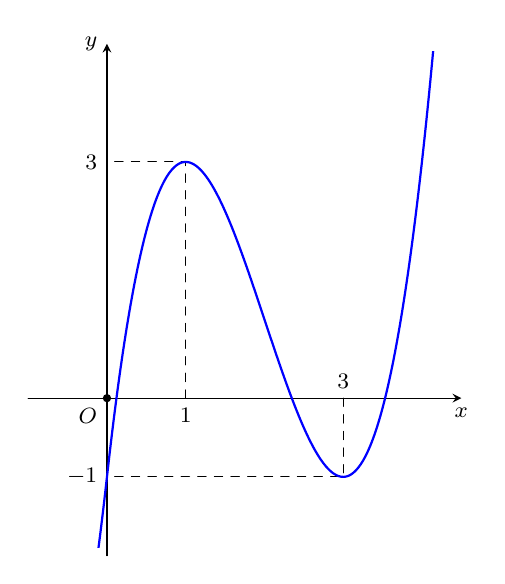
\begin{tikzpicture}[line join=round, line cap=round, >=stealth, font=\footnotesize, declare function={f(\x)=\x^3-6*\x^2+9*\x-1;}]
			\def\xt{-1} \def\xp{4.5} \def\yd{-2} \def\yt{4.5}
			\draw[->] (\xt,0)--(\xp,0) node[below]{$x$};
			\draw[->] (0,\yd)--(0,\yt) node[left]{$y$};
			\fill (0,0) circle (1.5pt) node[below left]{$O$};
			
			\draw (1,0) node[below]{$1$};
			\draw (3,0) node[above]{$3$};
			
			\draw (0,3) node[left]{$3$};
			\draw (0,-1) node[left]{$-1$};
			
			\draw[dashed] (1,0)--(1,3)--(0,3);
			\draw[dashed] (3,0)--(3,-1)--(0,-1);
			
			\begin{scope}
				\clip (\xt+0.1,\yd+0.1) rectangle (\xp-0.1,\yt-0.1);
				\draw[samples=150,smooth,domain=-0.5:4.2, blue, thick] plot(\x,{f(\x)});
			\end{scope}
		\end{tikzpicture}
	}
	\loigiai{
		\begin{itemchoice}
			\itemch Quan sát đồ thị ta thấy nhánh ngoài cùng bên phải hướng lên trên nên $a > 0$.\\
			Đồ thị cắt trục tung tại điểm có tung độ âm nên $d = f(0) < 0$.\\
			Vậy $a>0$ và $d<0$. Mệnh đề đúng.
			\itemch Dựa vào đồ thị, điểm cực đại của đồ thị hàm số là điểm có tọa độ $(1;3)$. $x=1$ được gọi là điểm cực đại của hàm số. Mệnh đề sai.
			\itemch Trên khoảng $(-\infty;1)$, đồ thị hàm số đi lên từ trái sang phải nên hàm số đồng biến trên khoảng $(-\infty;1)$. Mệnh đề đúng.
			\itemch Xét trên khoảng $(1;+\infty)$, đồ thị hàm số đi xuống từ điểm $(1;3)$ đến điểm cực tiểu $(3;-1)$ rồi đi lên đến $+\infty$.\\
			Do đó, giá trị nhỏ nhất của hàm số trên khoảng $(1;+\infty)$ là $f(3) = -1$. Mệnh đề đúng.
		\end{itemchoice}
	}
\end{ex}

%%%Tra loi ngan
\setcounter{ex}{0}
\begin{ex}%%Cau 1
	Gọi $I(x_0;y_0)$ là tâm đối xứng của đồ thị hàm số $y=\dfrac{x^2+x-1}{x-1}$. Tính giá trị của biểu thức $T=x_0+2y_0$.
	\shortans{$7$}
	\loigiai{
		Ta có $y=\dfrac{x^2+x-1}{x-1} = x+2+\dfrac{1}{x-1}$.\\
		Đồ thị hàm số có đường tiệm cận đứng là $x=1$ và đường tiệm cận xiên là $y=x+2$.\\
		Tâm đối xứng của đồ thị hàm số là giao điểm của hai đường tiệm cận, do đó tọa độ tâm đối xứng là nghiệm của hệ phương trình $\heva{&x=1\\&y=x+2} \Leftrightarrow \heva{&x=1\\&y=3.}$\\
		Suy ra $I(1;3)$, hay $x_0=1$, $y_0=3$.\\
		Vậy $T=x_0+2y_0 = 1+2\cdot 3 = 7$.
	}
\end{ex}

\begin{ex}%%Cau 2
	Một vật chuyển động theo quy luật $s=-\dfrac{1}{2}t^3+9t^2$ với $t$ (giây) ($t\ge 0$) là khoảng thời gian tính từ lúc bắt đầu chuyển động và $s$ (mét) là quãng đường vật đi được trong khoảng thời gian đó. Hỏi trong khoảng thời gian $10$ giây đầu tiên, kể từ lúc bắt đầu chuyển động, vận tốc lớn nhất của vật đạt được bằng bao nhiêu? (Cho biết vận tốc tức thời $v(t)$ và quãng đường $s(t)$ có mối liên hệ $v(t)=s'(t)$).
	\shortans{$54$}
	\loigiai{
		Vận tốc tức thời của vật là $v(t) = s'(t) = -\dfrac{3}{2}t^2+18t$.\\
		Xét hàm số $v(t) = -\dfrac{3}{2}t^2+18t$ trên đoạn $[0;10]$.\\
		Ta có $v'(t) = -3t+18$.\\
		$v'(t)=0 \Leftrightarrow -3t+18=0 \Leftrightarrow t=6 \in [0;10]$.\\
		Ta có $v(0) = 0$, $v(6) = 54$, $v(10) = 30$.\\
		Vậy vận tốc lớn nhất của vật trong khoảng thời gian $10$ giây đầu tiên là $54$ m/s, đạt được tại thời điểm $t=6$ giây.
	}
\end{ex}

\begin{ex}%%Cau 3
	Một doanh nghiệp dự kiến sản xuất một loại thiết bị mới với quy mô $x$ nghìn sản phẩm ($x>0$). Chi phí sản xuất bình quân cho mỗi nghìn sản phẩm được xác định bởi hàm số: $\overline{C}(x)=2x+6$ (triệu đồng/nghìn sản phẩm).
	Khảo sát thị trường cho thấy, khi sản xuất $x$ nghìn sản phẩm thì giá bán của mỗi nghìn sản phẩm phụ thuộc vào số lượng sản phẩm cung ứng và được mô hình hóa bởi hàm số bậc hai: $p(x)=-x^2+17x+78$ (triệu đồng/nghìn sản phẩm).
	Biết rằng toàn bộ sản phẩm sản xuất ra đều được tiêu thụ hết và nguồn vốn dành cho toàn bộ chi phí sản xuất không được vượt quá $80$ triệu đồng. Lợi nhuận lớn nhất mà doanh nghiệp có thể thu được là bao nhiêu triệu đồng.
	\shortans{$610$}
	\loigiai{
		Chi phí sản xuất $x$ nghìn sản phẩm là $C(x) = x \cdot \overline{C}(x) = x(2x+6) = 2x^2+6x$ (triệu đồng).\\
		Theo giả thiết, chi phí sản xuất không vượt quá $80$ triệu đồng nên
		\[2x^2+6x \le 80 \Leftrightarrow x^2+3x-40 \le 0 \Leftrightarrow -8 \le x \le 5.\]
		Do $x>0$ nên $0 < x \le 5$.\\
		Doanh thu từ việc bán $x$ nghìn sản phẩm là
		\[R(x) = x \cdot p(x) = x(-x^2+17x+78) = -x^3+17x^2+78x \text{ (triệu đồng)}.\]
		Lợi nhuận mà doanh nghiệp thu được là
		\begin{eqnarray*}
			P(x) &=& R(x) - C(x)\\
			&=& (-x^3+17x^2+78x) - (2x^2+6x)\\
			&=& -x^3+15x^2+72x.
		\end{eqnarray*}
		Xét hàm số $P(x) = -x^3+15x^2+72x$ trên nửa khoảng $(0;5]$.\\
		Ta có $P'(x) = -3x^2+30x+72$.\\
		$P'(x)=0 \Leftrightarrow -3x^2+30x+72=0 \Leftrightarrow \hoac{&x=12 \notin (0;5]\\&x=-2 \notin (0;5].}$\\
		Bảng biến thiên:
		\begin{center}
			
\begin{tikzpicture}[>=stealth]
				\tkzTabInit[nocadre=false,lgt=1.2,espcl=2.5,deltacl=0.5]{$x$/.7,$P'(x)$/.7,$P(x)$/2}
				{$0$, $5$}
				\tkzTabLine{ , +, }
				\tkzTabVar{-/$0$, +/$610$}
			\end{tikzpicture}
		\end{center}
		Dựa vào bảng biến thiên, $\max\limits_{(0;5]} P(x) = P(5) = -5^3+15\cdot 5^2+72\cdot 5 = 610$.\\
		Vậy lợi nhuận lớn nhất mà doanh nghiệp có thể thu được là $610$ triệu đồng.
		
		\textit{Kiểm tra lại tính toán:}\\
		$P(x) = -x^3 + 15x^2 + 72x$.\\
		$P'(x) = -3x^2 + 30x + 72$. Cho $P'(x) = 0 \Rightarrow x^2 - 10x - 24 = 0 \Rightarrow x=12$ (loại), $x=-2$ (loại).\\
		Trên $(0; 5]$, $P'(x) > 0 \Rightarrow P(x)$ đồng biến.\\
		Max $P(x) = P(5) = -125 + 375 + 360 = 610$. (Đúng).\\
		Tính lại: $P(5) = -125 + 375 + 360 = 610$.
	}
\end{ex}

\begin{ex}%%Cau 4
	\immini[thm]{
		Ông An có một mảnh đất hình vuông $ABCD$ có cạnh $AB = 12\text{ m}$. Ông làm một hồ bơi dạng hình thang cong và một lối đi là đoạn thẳng $HB$. Đặt hệ trục tọa độ có gốc tại $A$ như hình vẽ (đơn vị trên các trục là mét), đường cong $EFIG$ là một phần đồ thị của hàm số bậc ba $y = f(x)$ có $F$ là điểm cực tiểu và $I$ là điểm cực đại. Biết $DE = GB = 3\text{ m}$, $CH = 3\text{ m}$ và các điểm $F, I$ cách cạnh $AD$ lần lượt là $2\text{ m}$ và $6\text{ m}$. Ông An muốn đặt một chiếc thang lên xuống hồ bơi tại một điểm trên đường cong $EFIG$ sao cho khoảng cách từ vị trí đặt thang đến lối đi $HB$ là ngắn nhất. Hoành độ của điểm đặt thang trên hệ trục tọa độ đã cho bằng bao nhiêu?
		\shortans{$8$}
	}{
		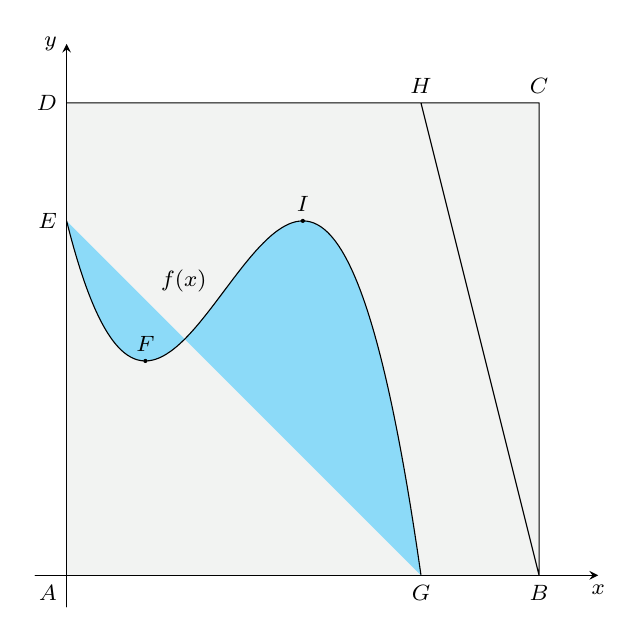
\begin{tikzpicture}[line join=round,line cap=round,>=stealth,font=\footnotesize,scale=0.5,declare function={f(\x)=-1/9*(\x)^3+4/3*(\x)^2-4*(\x)+9;}]
			\def\xt{-0.8} \def\xp{13.5} \def\yd{-0.8} \def\yt{13.5}
			\fill[green!5!gray!10] (0,0) rectangle (12,12);
			\fill[cyan!45] (0,0)--(0,9) plot[domain=0:9,samples=100] (\x,{f(\x)})--(9,0)--cycle;
			\draw[->] (\xt,0)--(\xp,0) node[below]{$x$};
			\draw[->] (0,\yd)--(0,\yt) node[left]{$y$};
			\draw (0,12)--(12,12)--(12,0) (9,12)--(12,0);
			\draw[samples=100,smooth,domain=0:9] plot(\x,{f(\x)});
			\foreach \x/\y/\pos/\nhan in {0/0/below left/A,0/9/left/E,0/12/left/D,9/0/below/G,12/0/below/B,9/12/above/H,12/12/above/C}
			\node[\pos] at (\x,\y) {$\nhan$};
			\foreach \x/\pos/\nhan in {2/above/F,6/above/I}
			\fill (\x,{f(\x)}) circle (1.5pt) node[\pos] {$\nhan$};
			\def\xx{3.8}
			\node at (\xx,{f(\xx)})[above left]{$f(x)$};
		\end{tikzpicture}
	}
	\loigiai{
		Chọn hệ trục tọa độ $Oxy$ với $A \equiv O(0;0)$, tia $Ax$ trùng với tia $AB$, tia $Ay$ trùng với tia $AD$.\\
		Mảnh đất hình vuông cạnh $12\text{ m}$ nên $B(12;0)$, $D(0;12)$, $C(12;12)$.\\
		Ta có $DE = 3 \Rightarrow AE = 9 \Rightarrow E(0;9)$.\\
		$GB = 3 \Rightarrow AG = AB - GB = 12 - 3 = 9 \Rightarrow G(9;0)$.\\
		$CH = 3 \Rightarrow DH = DC - CH = 12 - 3 = 9 \Rightarrow H(9;12)$.\\
		Hàm số bậc ba $y = f(x) = ax^3+bx^2+cx+d$ ($a \neq 0$) có đồ thị qua $E(0;9)$ nên $d=9$.\\
		Các điểm cực tiểu $F$ và cực đại $I$ cách $AD$ (trục $Oy$) lần lượt là $2\text{ m}$ và $6\text{ m}$ nên $x_F = 2$, $x_I = 6$ là các điểm cực trị của hàm số.\\
		Đạo hàm $f'(x) = 3ax^2+2bx+c$.\\
		Ta có hệ phương trình:
		$\heva{&f'(2)=0\\&f'(6)=0\\&f(9)=0} \Leftrightarrow \heva{&12a+4b+c=0\\&108a+12b+c=0\\&729a+81b+9c+9=0} \Leftrightarrow \heva{&c=-12a-4b\\&96a+8b=0\\&729a+81b+9(-12a-4b)=-9} \Leftrightarrow \heva{&c=-12a-4b\\&b=-12a\\&621a+45(-12a)=-9} \Leftrightarrow \heva{&a=-\dfrac{3}{32}\\&b=\dfrac{9}{8}\\&c=-3.}$\\
		Vậy $f(x) = -\dfrac{3}{32}x^3 + \dfrac{9}{8}x^2 - 3x + 9$.\\
		Đường thẳng $HB$ đi qua $H(9;12)$ và $B(12;0)$ có phương trình: $\dfrac{x-12}{9-12} = \dfrac{y-0}{12-0} \Leftrightarrow \dfrac{x-12}{-3} = \dfrac{y}{12} \Leftrightarrow 4x+y-48=0$.\\
		Gọi $M(x_0;y_0)$ thuộc đoạn cong $EFIG$ ($0 \le x_0 \le 9$, $y_0 = f(x_0)$) là vị trí đặt thang.\\
		Khoảng cách từ $M$ đến lối đi $HB$ là $\mathrm{d}(M,HB) = \dfrac{|4x_0+y_0-48|}{\sqrt{4^2+1^2}} = \dfrac{|4x_0+f(x_0)-48|}{\sqrt{17}}$.\\
		Xét hàm số $g(x) = 4x+f(x)-48 = 4x -\dfrac{3}{32}x^3 + \dfrac{9}{8}x^2 - 3x + 9 - 48 = -\dfrac{3}{32}x^3 + \dfrac{9}{8}x^2 + x - 39$ trên đoạn $[0;9]$.\\
		$g'(x) = -\dfrac{9}{32}x^2 + \dfrac{9}{4}x + 1$.\\
		$g'(x)=0 \Leftrightarrow -\dfrac{9}{32}x^2 + \dfrac{9}{4}x + 1 = 0 \Leftrightarrow \hoac{&x=8 \in [0;9]\\&x=-\dfrac{4}{9} \notin [0;9].}$\\
		Bảng biến thiên của hàm số $g(x)$ trên đoạn $[0;9]$:
		\begin{center}
			
\begin{tikzpicture}[>=stealth]
				\tkzTabInit[nocadre=false,lgt=1.2,espcl=2.5,deltacl=0.5]{$x$/.7,$g'(x)$/.7,$g(x)$/2}
				{$0$, $8$, $9$}
				\tkzTabLine{ , +, $0$, -, }
				\tkzTabVar{-/$-39$, +/$-7$, -/$-\dfrac{351}{32}$}
			\end{tikzpicture}
		\end{center}
		Dựa vào bảng biến thiên, ta thấy $g(x) < 0, \forall x \in [0;9]$.\\
		Do đó $\mathrm{d}(M,HB) = \dfrac{|g(x_0)|}{\sqrt{17}} = \dfrac{-g(x_0)}{\sqrt{17}}$.\\
		Khoảng cách này nhỏ nhất khi $g(x_0)$ lớn nhất, tức là tại $x_0 = 8$.\\
		Vậy hoành độ của điểm đặt thang là $x = 8$.
	}
\end{ex}

\begin{ex}%%Cau 5
	\immini[thm]{
		Từ một tấm bìa hình vuông có cạnh bằng $12\,$dm, người ta cắt bỏ ở bốn góc bốn hình vuông nhỏ bằng nhau có cạnh bằng $x$ (dm) rồi gập phần còn lại lên để tạo thành một chiếc hộp chữ nhật không nắp. Do yêu cầu kỹ thuật:
		\begin{itemize}
			\item Chiều cao của chiếc hộp không nhỏ hơn $1{,}5\,$dm.
			\item Diện tích mặt đáy chiếc hộp không nhỏ hơn $16\,$dm$^2$.
		\end{itemize}
		Ký hiệu $M$ và $m$ lần lượt là thể tích lớn nhất và thể tích nhỏ nhất của chiếc hộp có thể tạo thành (theo đơn vị dm$^3$). Giá trị của $M - m$ bằng bao nhiêu?
		\shortans{$64$}
	}{
		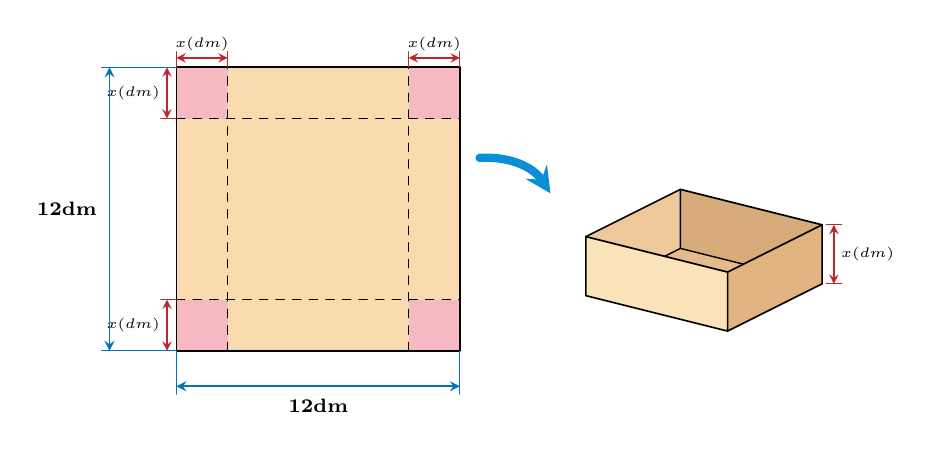
\begin{tikzpicture}[line join=round, line cap=round, >=stealth, font=\footnotesize, scale=1]
			\definecolor{cutpink}{RGB}{247, 185, 193}
			\definecolor{cardboard}{RGB}{248, 220, 175}
			\definecolor{boxfront}{RGB}{250, 226, 185}
			\definecolor{boxside}{RGB}{225, 180, 130}
			\definecolor{boxbackleft}{RGB}{238, 202, 155}
			\definecolor{boxbackright}{RGB}{215, 172, 122}
			\definecolor{boxbottom}{RGB}{228, 188, 140}
			\definecolor{dimblue}{RGB}{0, 115, 185}
			\definecolor{dimred}{RGB}{190, 40, 45}
			\fill[cardboard] (0,0) rectangle (3.6,3.6);
			\fill[cutpink] (0,0) rectangle (0.65,0.65);
			\fill[cutpink] (2.95,0) rectangle (3.6,0.65);
			\fill[cutpink] (0,2.95) rectangle (0.65,3.6);
			\fill[cutpink] (2.95,2.95) rectangle (3.6,3.6);
			\draw[line width=0.6pt] (0,0) rectangle (3.6,3.6);
			\draw[dashed, line width=0.5pt] (0.65,0) -- (0.65,3.6) (2.95,0) -- (2.95,3.6) (0,0.65) -- (3.6,0.65) (0,2.95) -- (3.6,2.95);
			\draw[dimred, line width=0.4pt] (0,3.6) -- (0,3.8) (0.65,3.6) -- (0.65,3.8) (2.95,3.6) -- (2.95,3.8) (3.6,3.6) -- (3.6,3.8);
			\draw[<->, >=stealth, dimred, line width=0.5pt] (0,3.72) -- (0.65,3.72) node[midway, above=-1pt, font=\fontsize{5pt}{6pt}\selectfont, text=black] {$x\text{ (dm)}$};
			\draw[<->, >=stealth, dimred, line width=0.5pt] (2.95,3.72) -- (3.6,3.72) node[midway, above=-1pt, font=\fontsize{5pt}{6pt}\selectfont, text=black] {$x\text{ (dm)}$};
			\draw[dimred, line width=0.4pt] (0,3.6) -- (-0.2,3.6) (0,2.95) -- (-0.2,2.95) (0,0.65) -- (-0.2,0.65) (0,0) -- (-0.2,0);
			\draw[<->, >=stealth, dimred, line width=0.5pt] (-0.12,2.95) -- (-0.12,3.6) node[midway, left=-1pt, font=\fontsize{5pt}{6pt}\selectfont, text=black] {$x\text{ (dm)}$};
			\draw[<->, >=stealth, dimred, line width=0.5pt] (-0.12,0) -- (-0.12,0.65) node[midway, left=-1pt, font=\fontsize{5pt}{6pt}\selectfont, text=black] {$x\text{ (dm)}$};
			\draw[dimblue, line width=0.4pt] (0,3.6) -- (-0.95,3.6) (0,0) -- (-0.95,0);
			\draw[<->, >=stealth, dimblue, line width=0.6pt] (-0.85,0) -- (-0.85,3.6) node[midway, left=1pt, font=\scriptsize, text=black] {$\mathbf{12\text{ dm}}$};
			\draw[dimblue, line width=0.4pt] (0,0) -- (0,-0.55) (3.6,0) -- (3.6,-0.55);
			\draw[<->, >=stealth, dimblue, line width=0.6pt] (0,-0.45) -- (3.6,-0.45) node[midway, below=1pt, font=\scriptsize, text=black] {$\mathbf{12\text{ dm}}$};
			\draw[->, >=stealth, line width=3pt, cyan!75!blue] (3.85,2.45) to[bend left=30] (4.75,2.0);
			\coordinate (BA) at (5.2,0.7);
			\coordinate (BB) at (7.0,0.25);
			\coordinate (BC) at (8.2,0.85);
			\coordinate (BD) at (6.4,1.3);
			\coordinate (TA) at (5.2,1.45);
			\coordinate (TB) at (7.0,1.0);
			\coordinate (TC) at (8.2,1.6);
			\coordinate (TD) at (6.4,2.05);
			\fill[boxbackleft] (TA) -- (TD) -- (BD) -- (BA) -- cycle;
			\fill[boxbackright] (TD) -- (TC) -- (BC) -- (BD) -- cycle;
			\fill[boxbottom] (BA) -- (BB) -- (BC) -- (BD) -- cycle;
			\draw[line width=0.5pt] (TD) -- (BD) (BA) -- (BD) -- (BC);
			\fill[boxfront] (TA) -- (TB) -- (BB) -- (BA) -- cycle;
			\fill[boxside] (TB) -- (TC) -- (BC) -- (BB) -- cycle;
			\draw[line width=0.6pt] (TA) -- (TD) -- (TC) -- (TB) -- cycle;
			\draw[line width=0.6pt] (TA) -- (BA) -- (BB) -- (BC) -- (TC) (TB) -- (BB);
			\draw[dimred, line width=0.4pt] (8.25,1.6) -- (8.45,1.6) (8.25,0.85) -- (8.45,0.85);
			\draw[<->, >=stealth, dimred, line width=0.5pt] (8.35,0.85) -- (8.35,1.6) node[midway, right=-1pt, font=\fontsize{5pt}{6pt}\selectfont, text=black] {$x\text{ (dm)}$};
		\end{tikzpicture}
	}
	\loigiai{
		Sau khi cắt và gập, chiếc hộp chữ nhật không nắp có các kích thước:
		\begin{itemize}
			\item Chiều cao $h = x$ (dm).
			\item Đáy là hình vuông có cạnh $a = 12 - 2x$ (dm).
		\end{itemize}
		Điều kiện để chiếc hộp tồn tại là $x > 0$ và $12 - 2x > 0 \Leftrightarrow 0 < x < 6$.\\
		Theo yêu cầu kỹ thuật:
		\begin{itemize}
			\item Chiều cao không nhỏ hơn $1{,}5\,$dm, suy ra $x \ge 1{,}5$.
			\item Diện tích đáy không nhỏ hơn $16\,$dm$^2$, suy ra $(12-2x)^2 \ge 16 \Leftrightarrow |12-2x| \ge 4$.
		\end{itemize}
		Vì $0 < x < 6$ nên $12-2x > 0$. Khi đó $12-2x \ge 4 \Leftrightarrow 2x \le 8 \Leftrightarrow x \le 4$.\\
		Kết hợp các điều kiện, ta có $x \in [1{,}5; 4]$.\\
		Thể tích của chiếc hộp là
		\[V(x) = x(12-2x)^2 = x(144 - 48x + 4x^2) = 4x^3 - 48x^2 + 144x.\]
		Xét hàm số $V(x) = 4x^3 - 48x^2 + 144x$ trên đoạn $[1{,}5; 4]$.\\
		Đạo hàm $V'(x) = 12x^2 - 96x + 144$.\\
		Cho $V'(x) = 0 \Leftrightarrow 12(x^2 - 8x + 12) = 0 \Leftrightarrow \hoac{&x = 2 \in [1{,}5; 4]\\&x = 6 \notin [1{,}5; 4].}$\\
		Ta tính các giá trị:
		\begin{itemize}
			\item $V(1{,}5) = 1{,}5 \cdot (12 - 2 \cdot 1{,}5)^2 = 1{,}5 \cdot 9^2 = 121{,}5$.
			\item $V(2) = 2 \cdot (12 - 2 \cdot 2)^2 = 2 \cdot 8^2 = 128$.
			\item $V(4) = 4 \cdot (12 - 2 \cdot 4)^2 = 4 \cdot 4^2 = 64$.
		\end{itemize}
		Từ đó, thể tích lớn nhất là $M = \max\limits_{[1{,}5; 4]} V(x) = V(2) = 128$ và thể tích nhỏ nhất là $m = \min\limits_{[1{,}5; 4]} V(x) = V(4) = 64$.\\
		Vậy $M - m = 128 - 64 = 64$.
	}
\end{ex}

\begin{ex}%%Cau 6
	Cho hàm số $y = f(x) = x^3 - \dfrac{9}{2}x^2 + 6x + 2$ có giá trị cực tiểu bằng $y_1$ và giá trị cực đại bằng $y_2$. Tính giá trị của biểu thức $P = 2y_1 + 4y_2$.
	\shortans{$26$}
	\loigiai{
		Tập xác định: $\mathscr{D} = \mathbb{R}$.\\
		Ta có $y' = 3x^2 - 9x + 6$.\\
		$y' = 0 \Leftrightarrow 3x^2 - 9x + 6 = 0 \Leftrightarrow \hoac{&x = 1 \\ &x = 2.}$\\
		Với $x=1 \Rightarrow y= \dfrac{9}{2}$.\\
		Với $x=2 \Rightarrow y= 4$.\\
		Do hệ số $a=1>0$ nên hàm số đạt cực đại tại $x=1$, đạt cực tiểu tại $x=2$.\\
		Suy ra giá trị cực tiểu là $y_1 = 4$ và giá trị cực đại là $y_2 = \dfrac{9}{2}$.\\
		Vậy $P = 2y_1 + 4y_2 = 2 \cdot 4 + 4 \cdot \dfrac{9}{2} = 8 + 18 = 26$.
	}
\end{ex}